\chapter{Rischio immobiliare}
\label{chap:secondo}
\section{Premessa}
\label{sec:prem}
Questo capitolo mira ad evidenziare gli aspetti pratici e tecnici più rilevanti nell'analisi di uno specifico rischio fra quelli contenuti nella vasta e complessa direttiva {\itshape Solvency II}. Per raggiungere al meglio tale fine si è rivelato quindi preferibile focalizzare l'attenzione su un solo oggetto d'analisi anziché offrire una panoramica su un numero maggiore di rischi a scapito del dettaglio di analisi.
Il rischio che si è scelto di analizzare è il {\itshape property risk} che costituisce, assieme ad altri descritti nella direttiva, una delle unità fondamentali per la costruzione del {\itshape SCR}. 
Come si vedrà nei paragrafi successivi, questo rischio coinvolge una parte di primaria importanza dell'attività assicurativa e riguarda elementi la cui valutazione è altamente condizionata dal livello di informazione di cui si dispone: gli immobili.
\section{Aspetti tecnici del {\itshape SCR}}
Il processo che ha portato alla direttiva {\itshape Solvency II} ha richiesto un lavoro a più livelli condotto sia da organi comunitari che nazionali (vedi \textit{supra} § \ref{subs:lamfalussy}). Gli aspetti tecnici principali sono stati definiti dall'EIOPA in un processo costante di comunicazione e aggiornamento con le autorità di vigilanza nazionali, le imprese assicurative e le loro associazioni.

\subsection{La struttura del {\itshape Solvency Capital Requirement}}
\label{subs:strutturascr}
Il {\itshape Solvency Capital Requirement} rappresenta il principale requisito quantitativo della Direttiva 2009/138/EC, sia per l'importanza che assume ai fini di vigilanza sia per la quantità di risorse necessarie alle imprese assicurative per il suo calcolo. La regolamentazione proposta da {\itshape Solvency II} si fonda su alcuni elementi fondamentali:
\begin{itemize}
\item una struttura di requisiti tripartita (quantitativi, qualitativi, informativi);
\item una valutazione a {\itshape fair valure} di tutte le poste di bilancio;
\item una valutazione delle riserve tecniche mediante il calcolo di {\itshape best estimate} e {\itshape risk margin};
\item un calcolo specifico dei requisiti di capitale e dei fondi propri.
\end{itemize}
Tali elementi rappresentano, con diversi gradi di differenziazione, un'innovazione rispetto alla precedente -- nonché vigente -- normativa, che, col progredire dell'innovazione degli strumenti finanziari e l'ampliamento dei settori di attività delle imprese assicurative, si è rivelata limitata.
Il {\itshape SCR} rappresenta da questo punto di vista uno degli elementi maggiormente potenziati, su richiesta sia delle autorità di vigilanza che delle imprese del settore, le quali lamentavano {\itshape in primis} una scarsa capacità di cogliere la rischiosità di un singolo fattore, di non considerare il tipo di attività e la dimensione della singola impresa \cite{cappiellorisk}. Le criticità del margine di solvibilità, ossia il vigente requisito di solvibilità, vengono attenuate solo in parte dalla maggiore facilità di calcolo, dovuta sia ad una effettiva semplicità dell'approccio sia ad una minore quantità di fattori da includere. \\
Il {\itshape SCR} proposto dalla direttiva {\itshape Solvency II} muta radicalmente l'approccio al problema della quantificazione dei requisiti di solvibilità definendo i rischi tipici delle categorie di attività delle imprese assicurative.

La misura di rischio scelta dall'autorità comunitaria per computare il {\itshape SCR} della singola  impresa assicurativa è il {\itshape Value at Risk} (v. {\itshape supra} § \ref{subs:SCR}). 
La soluzione ideata dal legislatore comunitario prevede che ogni categoria di rischio rappresenti un modulo composto a sua volta da sottorischi, dipendenti dall'operatività della singola impresa, la cui aggregazione conduce al {\itshape SCR} complessivo.
La figura \ref{fig:SCR} rappresenta l'ultima configurazione del {\itshape SCR}, proposta e valutata dall'EIOPA\footnote{L'ultima configurazione disponibile è quella usata per il quinto studio di impatto quantitativo (QIS5), i cui risultati sono stati pubblicati dall'Eiopa il 14 marzo 2011 \cite{reportqis5}.},  evidenziando la natura modulare del processo di calcolo del {\itshape SCR}. L'approccio modulare comprende sei rischi principali che compongono il {\itshape basic solvency capital requirement}, al quale occorre aggiungere il modulo per i rischi operativi per giungere al requisito di solvibilità generale.
\begin{figure}[htbp]
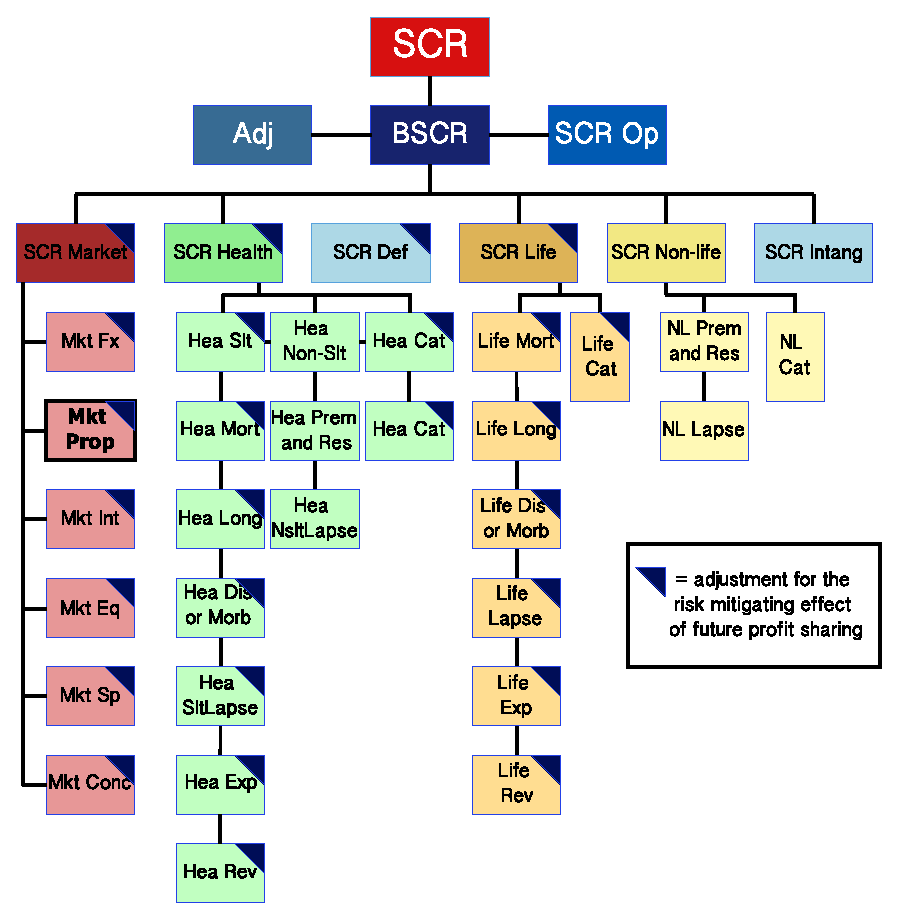
\includegraphics[scale=1]{Immagini/StrutturaSCR.eps}
\caption[Struttura del \textit{SCR}]{La struttura dei moduli e dei sottomoduli del Solvency Capital Requirement}
\label{fig:SCR}
\end{figure} 

Ogni categoria principale di rischio prevede sottorischi specifici per i settori in cui la singola compagnia opera: tali sottorischi vanno calcolati singolarmente e aggregati tramite una matrice di correlazione, che permette di considerare, nel calcolo complessivo, l'effetto di diversificazione. Un secondo effetto che il {\itshape SCR} considera, per costruzione, è quello della mitigazione del rischio derivante dal {\itshape profit sharing business}\footnote{In figura  \ref{fig:SCR} sono evidenziati i rischi per cui questo tipo di mitigazione del rischio è consentita.} e dal fondo per il differimento delle imposte.

\subsection{Il {\itshape property risk}: aspetti valutativi}
\label{subs:propertyrisk}
Una prima definizione del {\itshape property risk} viene data nella direttiva {\itshape Solvency II}\footnote{vedi art. 105, comma 5, lettera c.} che lo definisce come:
\begin{quotation} «[...] the sensitivity of the values of assets, liabilities and financial instruments to changes in the level or in the volatility of market prices of real estate».
\end{quotation}
Nelle misure di secondo livello, per lo sviluppo delle quali la commissione europea si avvale del contributo dell'EIOPA, la definizione del {\itshape property risk} cambia lievemente\footnote{La definizione nei {\itshape consulting papers} del CEIOPS diventa: «Property risk arises as a result of sensitivity of assets, liabilities and financial investments to the level or volatility of market prices of property» (\cite[p. 23]{eiopal2standardformula})}, pur mantenendo gli elementi essenziali che lo determinano.
Il {\itshape property risk} diventa quindi il livello di sensibilità che attivi, passivi e attività finanziarie hanno nei confronti del livello o della volatilità dei prezzi di mercato. L'approccio per la valutazione di tale rischio è di tipo $\Delta$-NAV: si presume uno shock di ammontare arbitrario\footnote{Questi valori sono attualmente in fase di studio e di \textit{testing} da parte delle autorità europee: nell'ultimo studio di impatto quantitativo, il quinto, l'EIOPA raccomanda di utilizzare uno shock non inferiore al 25\% \cite{eiopaqis5calibration}.} sul {\itshape net asset value} ({\itshape NAV}), ovvero la differenza fra attività e passività, sempre valutate in un'ottica {\itshape market consistent} (vedi \textit{supra} § \ref{subs:attepass}).
Possiamo sintetizzare in forma analitica il valore assunto dal requisito di solvibilità relativo al {\itshape property risk} come:

\begin{equation}
Mkt_{property} = max(\Delta NAV|_{25\%},0).
\label{for:propertyrisk}
\end{equation}
Tale formulazione poggia sull'ipotesi di uno scenario in cui il valore degli investimenti immobiliari diminuisca istantaneamente del 25\%. 
Il valore degli investimenti immobiliari è determinato dalla somma di diversi tipi di investimenti, per altro tipici dell'impresa assicurativa, esso è infatti camposo da:
\begin{itemize}
\item terreni, immobili e diritti su immobili;
\item partecipazioni (dirette o indirette) in società immobiliari che producono un reddito periodico;
\item investimenti immobiliari per l'uso proprio dell'impresa.
\end{itemize}
Per tale ragione vanno assoggettate al modello di calcolo del rischio azionario altri tipi di investimenti solo all'apparenza immobiliari, come:
\begin{itemize}
\item investimenti in società che si occupano di gestione immobiliare;
\item investimenti in società impegnate nello sivluppo di progetti immobiliari;
\item investimenti in società che hanno ricevuto prestiti da istituzioni esterne al gruppo assicurativo col fine si stimolare l'investimento in immobili.
\end{itemize}
La direttiva e le misure di secondo livello permettono, come esposto anche nella figura \ref{fig:SCR}, di ridurre il valore del fabbisogno di capitale per il {\itshape property risk} includendo nel calcolo eventuali fattori di assorbimento delle perdite.

\section{La valutazione degli immobili}
\label{sec:valimmobili}
Uno degli aspetti principali per la stima del {\itshape property risk} è il metodo di valutazione dei beni immobili detenuti dall'impresa assicurativa. 
L'approccio più diffuso in letteratura per la valutazione di un immobile prevede in prima istanza  di identificare i rendimenti attesi dal soggetto che opta per questa forma di investimento. In quest'ottica i rendimenti e il valore dell'immobile appaiono in stretta relazione fra loro, relazione che David Geltner definisce così (\cite[p. 202]{geltner}):
\begin{quotation}
«The prices investors pay for properties determine their expected returns, because the future cash flow the properties can yield is independent of the prices investors pay today for the properties».
\end{quotation}
Ciò significa che il prezzo corrisposto per l'acquisto di un immobile determina i rendimenti che l'acquirente si attende dal suo investimento, ma questi rimangono indipendenti dal prezzo iniziale.
La relazione che sussiste fra rendimenti attesi e valore dell'immobile, dato un certo prezzo di acquisto, risulta quindi essere inversa, in quanto i rendimenti futuri\footnote{nei rendimenti futuri viene incluso anche il prezzo al quale l'immobile verrà rivenduto} che l'investitore si aspetta di ricevere sono indipendenti nel tempo e sono svincolati dall'ammontare corrisposto per l'acquisto. Nello specifico i rendimenti attesi, che nella prassi corrispondono ai canoni di locazione, sono indipendenti poichè vengono determinati dall'incontro fra domanda e offerta degli immobili in locazione o, più semplicemente, dal mercato. L'indipendenza degli affitti dal prezzo corrisposto per l'acquisto dell'immobile influenza a sua volta il prezzo di vendita, poichè questo sarà, in un'ottica di continuità degli scambi, il prezzo di acquisto che il nuovo acquirente sarà disposto a pagare. Tale nuovo soggetto calcolerà il prezzo sulla base dei rendimenti attesi, ovvero delle potenziali entrate future derivanti da locazione.
\begin{figure}[htbp]
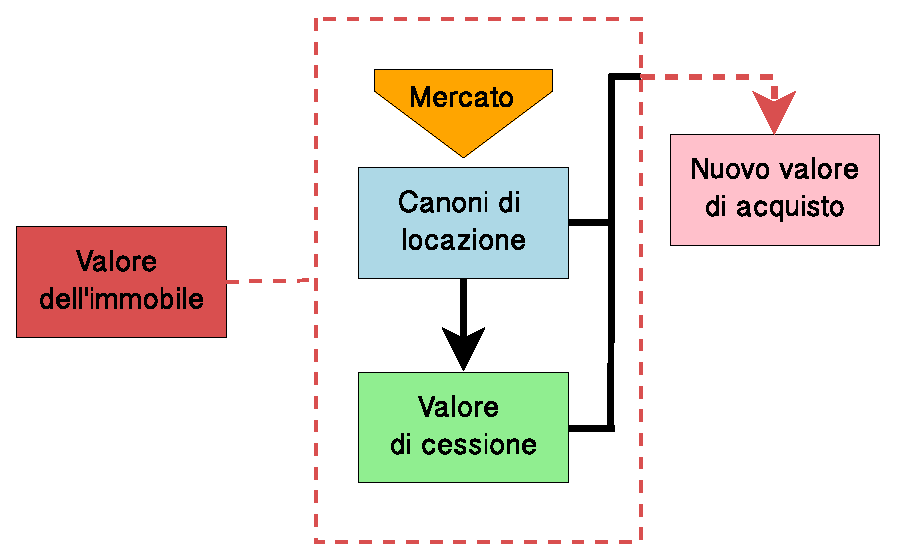
\includegraphics[scale=1]{Immagini/valoreimmobile.eps}
\caption[Sintesi della determinazione del valore di un immobile]{Il processo e le variabili che determinano il valore di un immobile}
\label{fig:valoreimmobile}
\end{figure} 

La figura \ref{fig:valoreimmobile} illustra il processo che viene compiuto ad ogni valutazione che coinvolge l'immobile di riferimento, evidenziando il ruolo svolto dal mercato nella determinzione dei canoni di locazione, variabile che assume un'importanza centrale nel metodo che si andrà ad illustrare.

\subsection{Discounted Cash Flow}
\label{subs:dcf}
Una delle procedure di valutazione più importanti nella microeconomia applicata al {\itshape real estate} è sicuramente il {\itshape multiperiod discounted cash flow} (da qui in avanti abbreviato in {\itshape DCF}). Questo sistema, utilizzato anche per lo svolgimento di questo lavoro, si sostanzia di tre momenti:
\begin{enumerate}
\item stimare i flussi di cassa attesi;
\item definire il rendimento totale che ci aspetta dall'invetimento immobiliare;
\item scontare al valore attuale i flussi di cassa al tasso di rendimento definito.
\end{enumerate}
Questi tre momenti si sostanziano analiticamente nella formula \ref{for:dcf}:
\begin{equation}
V = \frac{E_0[CF_1]}{1+E_0[r]} + \frac{E_0[CF_2]}{(1+E_0[r])^2} + \ldots + \frac{E_0[CF_{T-1}]}{(1+E_0[r])^{T-1}} + \frac{E_0[CF_T]}{(1+E_0[r])^T}.
\label{for:dcf}
\end{equation}
dove:
\begin{description}
\item $ V = $ valore attuale dell'immobile;
\item $ CF_{t} = $ flussi di cassa generati dall'immobile\footnote{nella prassi i flussi di cassa corrispondono alle cifre incassate dall'affitto dell'immobile di riferimento.} nel periodo $ t $;
\item $ E_0[r] = $ tasso medio atteso per periodo, che corrisponde al costo opportunità del capitale (da qui in poi \textit{OCC}\footnote{acronimo di {\itshape opportunity cost of capital}.}) dell'investimento immobiliare;
\item $ T = $ periodo finale dell'intera durata dell'investimento che, per convenzione, è anche il periodo in cui l'immobile verrà venduto.
\end{description}
Il valore attuale che deriva da questo sistema di calcolo si riferisce alle attese, riguardo flussi di cassa e rendimenti, del soggetto che effettua la stima. Tali attese potrebbero, in scenari come quelli di un mercato dove l'informazione non è completa e può essere asimmetrica, discostarsi dal valore effettivo a cui l'immobile potrebbe essere venduto. Se, per esempio, il risultato del calcolo secondo i \textit{DCF} fosse superiore all'effettivo prezzo di vendita, avremmo una situazione di guadagno per il venditore e perdita, in termini di costo opportunità\footnote{questo perchè il rendimento atteso del compratore sarebbe in realtà inferiore a quello utilizzato per i calcoli.}, per il compratore\footnote{il risultato sarebbe invertito qualora il valore individuato con il metodo dei \textit{DCF} fosse fosse inferiore prezzo di vendita.}.

\subsection{L'\textit{OCC} come fattore di rischio}
\label{subs:occ}
Il modello dei \textit{DCF} si basa su stime che spesso sono affidate alle capacità e alla sensibilità dell'analista; in particolare appare ragionevolmente complicato riuscire a stimare con precisione l'\textit{OCC}, che, per giunta, mutando nel tempo, dovrebbe tendere ad un incremento, rappresentativo di un aumento di rischio, per i flussi di cassa più lontani. L'\textit{OCC}, che ha la funzione di convertire un valore futuro (i flussi di cassa) in un valore corrente, è un fattore rappresentativo di due rischi distinti: da un lato il rischio insito nel variare del valore del denaro nel tempo, dall'altro quello che i flussi di cassa più distanti non si trasformino in canoni effettivamente riscossi.
Il tasso di rendimento ($ E_0[r] $ della \ref{for:dcf}, p. \pageref{for:dcf}) può essere quindi visto come somma di due componenti principali: una componente {\itshape risk-free} e una di premio di rischio (o {\itshape risk premium}). 
\begin{equation}
r = r_f + RP.
\label{for:r}
\end{equation}
La prima componente riguarda la variazione del valore del denaro nel tempo, mentre la seconda si riferisce al rischio che i flussi di cassa futuri non corrispondano ai flussi futuri reali.
Questa seconda parte di rischio è la più mutevole della somma descritta nella \ref{for:r}, poichè può essere ridimensionata in caso siano presenti dei contratti di locazione per i periodi cui il tasso di rendimento si riferisce. La presenza di un contratto permette di diminuire il rischio di un'asimmetria fra flussi attesi e flussi reali futuri, riducendo, in casi estremi, il rischio del rendimento alla sola parte {\itshape risk-free} ($ r_f $).

\subsection{L'{\itshape Interlease Discount Rate}}
\label{subs:idr}
Alla luce di quanto descritto nel paragrafo \ref{subs:occ} è necessario computare un secondo tasso di sconto da applicare a tutti i periodi successivo o al di fuori di quelli coperti da contratti di locazione: tale tasso consiste in un maggiore {\itshape risk premium} dovuto all'aumento del rischio derivante da flussi di cassa più incerti.
Questo rischio modifica sensibilmente la formula dei \textit{DCF} (\ref{for:dcf}) che possiamo riscrivere, inserendo il nuovo tasso $i$ ottenendo la \ref{for:dcfinter}.
Il nuovo tasso di sconto prende il nome di {\itshape interlease dicount rate}
\begin{equation}
V = \underbrace{\sum_{t=1}^{m} \frac{E_0[CF_1]}{1+E_0[r]}}_\textit{Periodi con contratti} + \underbrace{\underbrace{\left(\frac{1}{(1+E_0[i])^m}\right)}_\textit{Interlease DR} \cdot \underbrace{\left(\sum_{t=1}^{n-1} \frac{E_0[CF_{1}]}{(1+E_0[r])^{1}} \right)}_\textit{Periodi futuri}}_\textit{Periodi futuri privi di contratti di locazione} + \underbrace{\frac{E_0{CF_n}}{(1+E_0[i])^n}}_\textit{Valore di cessione} .
\label{for:dcfinter}
\end{equation}
dove i parametri sono i medesimi della \ref{for:dcf} e in aggiunta:
\begin{description}
\item $ i $ = {\itshape interlease discount rate};
\item $ m $ = ultimo periodo di applicazione di un tasso determinato dall'esistenza di un  contratto;
\item $ n $ = periodo finale della valutazione in cui si suppone la cessione dell'immobile.
\end{description}
Appare intuitivo constatare che l'{\itshape interlease discount rate} (da qui innanzi {\itshape IDR}) sarà, salvo casi eccezionali\footnote{un esempio in questo senso è il caso in cui si è certi di affittare l'immobile in un periodo successivo ai primi, ma a ben vedere si tratta di un numero assai limitato di casi.}, sempre maggiore dell'\textit{OCC} dei primi periodi, in quanto rappresentativo di un rischio maggiore dovuto all'incertezza di un evento futuro.

\subsection{Il {\itshape vacancy rate}}
\label{subs:vacancyrate}
Il {\itshape vacancy rate} è un fattore ampiamente usato in macroeconomia che esprime la percentuale di immobili non occupati sul totale di quelli disponibili. Questo dato, alla stregua di altri rapporti analoghi -- si pensi al tasso di disoccupazione -- assume per natura un valore diverso da zero, perchè, in termini di economicità, non è conveniente che un proprietario affitti un immobile al primo soggetto che lo richiede e, analogamente, non è conveniente per chi ricerca un immobile accettare la prima proposta. Tale non convenienza deriva dal fatto che ci sono dei costi per entrambe le parti alla stipula del contratto e dal basso costo della ricerca di offerte migliori: il tempo necessario per la ricerca di un immobile o di un conduttore genera il {\itshape vacancy rate}. Un altro motivo che giustifica l'esistenza di questo tasso è l'asimmetria nei tassi di crescita di domanda e offerta di immobili.
In generale il {\itshape vacancy rate} si attesta su un valore naturale dato dalla sua media nel lungo periodo.

Il {\itshape} vacancy rate può assume valori inferiori o superiori rispetto al suo valore naturale, e in entrambi i casi possiamo prevedere con buona approssimazione i cambiamenti nel mercato:
\begin{itemize}
\item se $vr > vr_n$, i canoni di affitto tenderanno a diminuire;
\item se $vr < vr_n$, i canoni di affitto tenderanno a crescere e potrebbe iniziare una fase espansiva dell'offerta (nuove costruzioni).
\end{itemize}

Nell'ambito del modello di seguito proposto (v. \textit{ultra} § \ref{sec:modello}), il {\itshape vacancy rate} assume una funzione analoga, ancorchè limitata ad un immobile. Come si avrà modo di analizzare nel § \ref{subs:datiinput}, il modello sviluppato utilizza dati relativi ad immobili composti da più locali (per ipotesi tutti uffici): in questo caso il {\itshape vacancy rate} indicherà la quantità di locali non affittati sul totale dei locali che compongono l'immobile.


\section{Modello proposto}
\label{sec:modello}
Il modello utilizzato nel prosieguo di questo lavoro è basato sul metodo dei \textit{DCF} (vedi \textit{supra} § \ref{subs:dcf}) ed è stato sviluppato con il \textit{software} MATLAB. Per un approfondimento sui codici del programma si rimanda all'appendice \ref{app:listatomatlab} (p. \pageref{app:listatomatlab}), mentre per i risultati dei diversi scenari si rimanda ai successivi paragrafi dove sono riportati in forma tabellare.

Data l'architettura del programma utilizzato e l'elevato numero di calcoli, è stato necessario -- e più agevole -- lavorare mediante una struttura matriciale, dove ogni variabile rappresentava una dimensione ulteriore e ogni vettore conteneva la serie di dati della variabile. Ogni matrice così costituita rappresenta un singolo immobile e il programma sviluppato usava in sequenza la matrice di ogni immobile, contenuta in un singolo input file.

\subsection{Dati in input}
\label{subs:datiinput}
Il programma sviluppato legge diversi dati di input, ma solo alcuni di essi sono fondamentali per il suo funzionamento:
\begin{itemize}
\item i flussi di cassa di ciascun periodo ($CF_i$);
\item il tasso di interesse, l'\textit{OCC} di ogni periodo ($E_0[r]$);
\item il valore stimato di vendita.
\end{itemize}
Rappresentano invece dati opzionali per il funzionameto del modello:
\begin{itemize}
\item l'{\itshape interlease discount rate};
\item il {\itshape vacancy rate}.
\end{itemize}
Un dato fondamentale, che il programma non richiede, è il numero di periodi di analisi; tale dato non è necessario in quanto il programma lo ricava da sé misurando la lunghezza del vettore dei flussi di cassa. Vale la pena ricordare che è necessario, affinchè il programma funzioni, avere vettori di uguale lunghezza.
Il cuore del programma è basato sulla formula \ref{for:dcfinter}, per tanto il valore di cessione dell'immobile è scorporato dal vettore dei flussi di cassa e si considerà come uno scalare (o vettore unitario).
Le serie storiche utilizzate per estrarre i dati appartengono a fonti diverse:
\begin{itemize}
\item per i flussi di cassa e il valore di vendita è stato utilizzato il database di {\itshape scenari immobiliari};
\item i tassi di interesse sono stati ricavati dai dati dell'{\itshape IPD} estratti dal database {\itshape Bloomberg}.
\end{itemize}
Per le analisi che hanno previsto l'utilizzo di \textit{IDR} e di {\itshape vacancy rates}:
\begin{itemize}
\item gli \textit{IDR} sono stati calcolati sulla base degli \textit{OCC} e secondo ipotesi;
\item i {\itshape vacancy rates} sono stati estratti dal database della Jonas Lang LaSalle.
\end{itemize}

I dati utilizzati per i calcoli sono tutti relativi ad immobili (composti ciascuno da un numero di uffici compreso fra le 20 e le 30 unità) selezionati nelle aree del centro e immediatamente limitrofe di cinque città italiane\footnote{i dati si riferiscono alle città di Milano, Roma, Torino, Bologna e Padova, per ulteriori specificazioni si rimanda all'Appendice \ref{app:datiimmobili}.}. La metratura media di ogni ufficio varia in funzione della città, come esposto nella tabella \ref{tab:metrature}.
\begin{table}[htbp]
\begin{center} \begin{tabular}{|c|c|c|}
\hline
{\bfseries Città} & {\bfseries Metratura media} & {\bfseries Uffici per immobile} \\
\hline
Milano & 200 & 20 \\
\hline
Roma & 100 & 20 \\
\hline
Torino & 90 & 25 \\
\hline
Bologna & 90 & 25 \\
\hline
Padova & 85 & 30\\
\hline
\end{tabular} \end{center}
\caption{Numero di uffici e metratura media distinti per città}
\label{tab:metrature}
\end{table}
Per una maggiore comparabilità dei risultati si è scelto di lavorare con i dati medi riportati nella tabella \ref{tab:metriufficimedi}:
\begin{table}[htbp]
\begin{center} \begin{tabular}{|c|c|c|}
\hline
{\bfseries Città} & {\bfseries Metratura media} & {\bfseries Uffici per immobile} \\
\hline
Tutte & 113 $\approx$ 115 & 24 $\approx$ 25 \\
\hline
\end{tabular} \end{center}
\caption{Valori medi di metratura e uffici}
\label{tab:metriufficimedi}
\end{table}
Tali ipotesi non hanno impatti rilevanti sui risultati finali e consentono una migliore percezione dei dati elaborati, in quanto un prezzo espresso al metro quadro o al metro quadro per anno è meno agevole da leggere più difficile da confrontare rispetto al valore dell'intero immobile.

\subsection{Risultati per lo scenario base}
\label{subs:risultatiscenbase}
Lo scenario basilare prevede l'applicazione del modello ai soli dati fondamentali descritti al paragrafo \ref{subs:datiinput}, vale a dire flussi di cassa, valore di cessione e rendimenti. In questa prima fase si suppone che gli immobili siano sempre affittati ({\itshape vacancy rate} nullo) e che tutti i contratti futuri siano già stati stipulati {\itshape IDR nullo}.
Nella tabella \ref{tab:dcfmirotobopd} sono riportati i risultati per singolo immobile raggruppati per città..

% Tabelle DCF Milano, Roma, Torino, Bologna, Padova
\begin{table}[htbp]
\begin{center} 
\begin{tabular}[c]{|l||c|}
\hline
{\bfseries Milano} & {\bfseries \textit{DCF}} \\
\hline \hline
Imm. 1 & 16.205.885 \\
\hline
Imm. 2 & 24.732.349 \\
\hline
Imm. 3 & 31.542.120 \\
\hline
Imm. 4 & 26.129.468 \\
\hline
\end{tabular}
\hspace{5mm}
\begin{tabular}[c]{|l||c|}
\hline
{\bfseries Roma} & {\bfseries \textit{DCF}} \\
\hline \hline
Imm. 1 & 38.120.230 \\
\hline
Imm. 2 & 26.640.321 \\
\hline
Imm. 3 & 24.548.218 \\
\hline
Imm. 4 & 22.257.105 \\ 
\hline
\end{tabular}
\hspace{5mm}
\vspace{1cm}
\begin{tabular}[c]{|l||c|}
\hline
{\bfseries Torino} & {\bfseries \textit{DCF}} \\
\hline \hline
Imm. 1 & 9.220.290 \\
\hline
Imm. 2 & 16.453.004 \\
\hline
Imm. 3 & 24.548.218 \\
\hline
Imm. 4 & 9.172.760 \\
\hline
\end{tabular} 
\hspace{5mm}
\begin{tabular}[c]{|l||c|}
\hline
{\bfseries Bologna} & {\bfseries \textit{DCF}} \\
\hline \hline
Imm. 1 & 15.439.025 \\
\hline
Imm. 2 & 13.411.647 \\
\hline
Imm. 3 & 15.168.141 \\
\hline
Imm. 4 & 14.600.870 \\
\hline
\end{tabular} 
\hspace{5mm}
\begin{tabular}[c]{|l||c|}
\hline
{\bfseries Padova} & {\bfseries \textit{DCF}} \\
\hline \hline
Imm. 1 & 13.124.147 \\
\hline
Imm. 2 & 13.946.266 \\
\hline
Imm. 3 & 12.469.543 \\
\hline
Imm. 4 & 13.140.184 \\
\hline
\end{tabular} 
\caption[DCF per gli immobili scelti]{DCF per gli immobili siti a Milano, Roma, Torino, Bologna e Padova}
\label{tab:dcfmirotobopd}
\end{center}
\end{table}

Si ricorda che i risultati sono calcolati sulla base delle ipotesi di metratura media e composizione degli immobili riportate al § \ref{subs:datiinput} e che i dati relativi ai canoni e all'ubicazione dei singoli immobili sono riportati in Appendice \ref{app:datiimmobili}.
L'\textit{OCC} utilizzato è il tasso medio dell'indice ISI di settore\footnote{nello specifico l'{\itshape Italy ISI Property Offices} reperibile su \textit{Bloomberg} con il \textit{Ticker} ITHPO.} elaborato da Scenari Immobiliari SpA, relativo agli ultimi dieci anni. I valori si intendono espressi in euro.
Di seguito, nella tabella \ref{tab:dcfbasedescrittive}, si evidenziano le principali statistiche descrittie sui dati prodotti dal modello aggregati per città.

% Tabella statistiche descrittive DCF Scenario Base
\begin{table}[htbp]
\label{tab:dcfbasedescrittive}
\begin{center}
\begin{tabular}[c]{|l||*{5}{c|}}
\hline
{\bfseries Città} & {\bfseries Obs} & {\bfseries Media DCF} & {\bfseries Std. Dev.} DCF & {\bfseries Min} & {\bfseries Max} \\
\hline \hline
Milano & 4 & 24.652.456 & 6350852,41 & 16.205.885 & 31.542.120 \\
\hline
Roma & 4 & 27.891.469 & 7050208,22 & 22.257.105,00 & 38.120.230 \\
\hline
Torino & 4 & 14.848.568 & 7315502,60 & 9.172.760 & 24.548.218 \\
\hline
Bologna & 4 & 14.654.921 & 899419,37 & 13.411.647 & 15.439.025 \\
\hline
Padova & 4 & 13.170.035 & 604488,87 & 12.469.543 & 13.946.266 \\
\hline
{\itshape Totale} & 20 & 19.043.490 & 7808886,69 & 9.172.760 & 38.120.230 \\
\hline
\end{tabular}
\caption{Principali statistiche descrittive sui dati prodotti dal modello}
\end{center}
\end{table}
